\chapter{Manual de usuario}
\label{cap:manual_usuario}

Este manual de usuario esta diseñado para proporcionar una guía completa sobre el uso de la aplicación desarrollada durante el Trabajo de Fin de Grado.
La aplicación esta dirigida principalmente a estudiantes y jóvenes trabajadores que comparten vivienda y busca facilitar la organización del hogar.


Este manual proporciona una explicación detallada de cada funcionalidad, acompañada de imágenes y pasos a seguir, con el objetivo de que el usuario pueda familiarizarse rápidamente con el funcionamiento de la aplicación, desde el registro inicial hasta el uso de sus herramientas principales.
Se recomienda leer este manual antes del primer uso de la aplicación, especialmente si se desea aprovechar todas sus funcionalidades de forma eficiente.

\section{Requisitos previos}
Antes de utilizar la aplicación, es necesario cumplir con los siguientes requisitos previos:

\begin{itemize}
    \item \textbf{Conexión a internet:} La aplicación requiere una buena conexión a internet para funcionar correctamente, debido a que utiliza servicios en la nube para almacenar y gestionar los datos.
    \item \textbf{Acceso a la aplicación:} Como la aplicación aún no esta publicada en ninguna tienda de aplicaciones, se debe acceder a través de un enlace web. El enlace proporcionado es el siguiente: \url{https://hogar-3f60f.web.app/} que nos proporciona acceso a la aplicación en modo web.
    \item \textbf{Correo electrónico activo:} Para registrarse en la aplicación, es necesario tener una dirección de correo electrónico válido, ya que necesitaremos verificar la cuenta mediante un enlace de confirmación enviado al correo electrónico proporcionado durante el registro.
    \item \textbf{Navegador compatible:} La aplicación es compatible con la mayoría de los navegadores modernos, como Google Chrome, Mozilla Firefox, Microsoft Edge y Safari. Se recomienda utilizar la última versión del navegador para garantizar un funcionamiento sin errores. 
\end{itemize}

\section{Registro e inicio de sesión}

Los primero que nos mostrará la aplicación al acceder a ella por primera vez, será la pantalla de bienvenida, 
donde se nos dará la bienvenida a la aplicación y se nos ofrecerá la opción de registrarnos o iniciar sesión si ya tenemos una cuenta creada.

\subsection*{Registro}

En el caso de que no tengamos una cuenta creada, debemos pulsar el botón de \textit{Registrarse} que nos llevará a la pantalla de registro.

\begin{figure}[H]
    \centering
        
\includegraphics[width=0.55\textwidth]{../capitulos/img/manual1.png}
        \caption{Opción de registrarse}
\end{figure}

En la pantalla de registro, debemos completar los siguientes campos: 

\begin{itemize}
    \item \textbf{Nombre:} Introduce tu nombre completo.
    \item \textbf{Apellidos:} Introduce tus apellidos.
    \item \textbf{Correo electrónico:} Introduce una dirección de correo electrónico válida, ya que se enviará un enlace de verificación a esta dirección.
    \item \textbf{Contraseña:} Introduce una contraseña segura que cumpla con los requisitos de seguridad (mínimo 6 caracteres).
\end{itemize}

Una vez completados todos los campos (es obligatorio rellenarlos todos), debemos pulsar el botón de "Registrarse" para crear nuestra cuenta.


\begin{figure}[H]
    \centering
        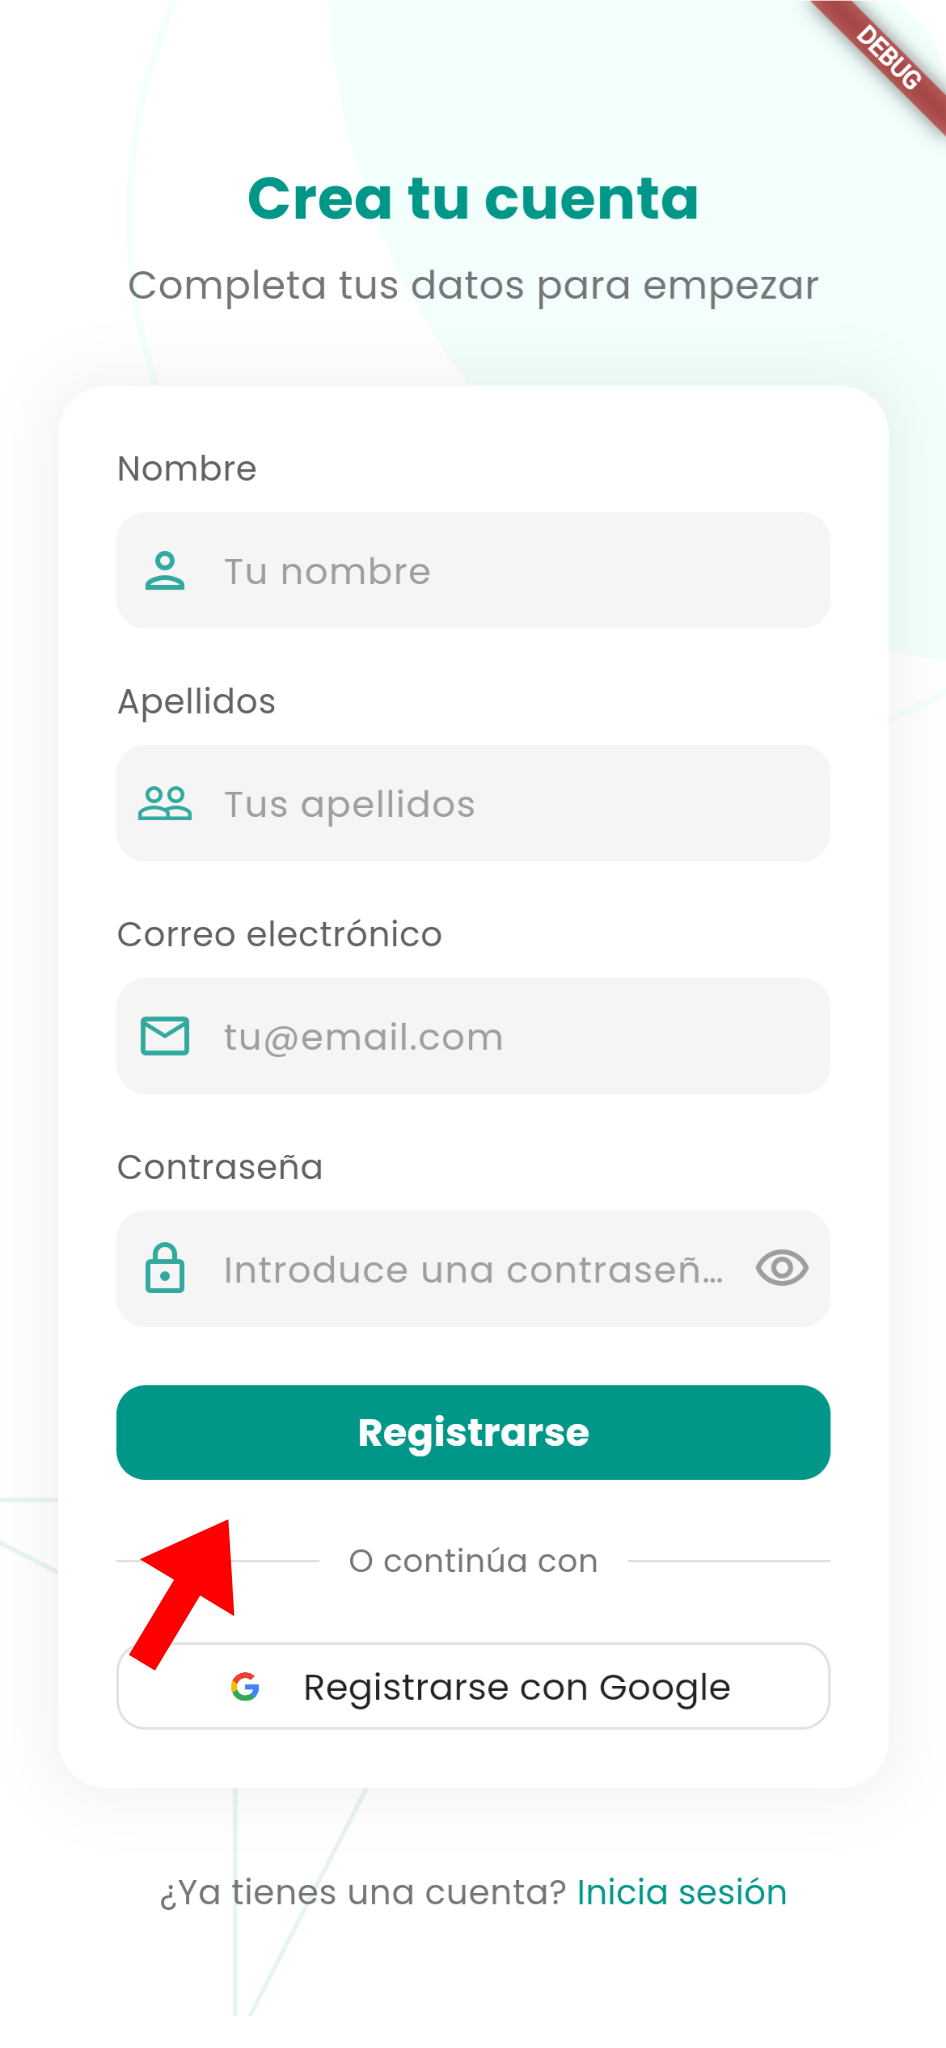
\includegraphics[width=0.55\textwidth]{../capitulos/img/manual2.png}
        \caption{Pantalla de registro de usuario}
\end{figure}

Una vez pulsado el botón de \textit{Registrarse}, se mostrará la siguiente pantalla y se enviará un correo electrónico a la dirección proporcionada con un enlace de verificación.

\begin{figure}[H]
    \centering
        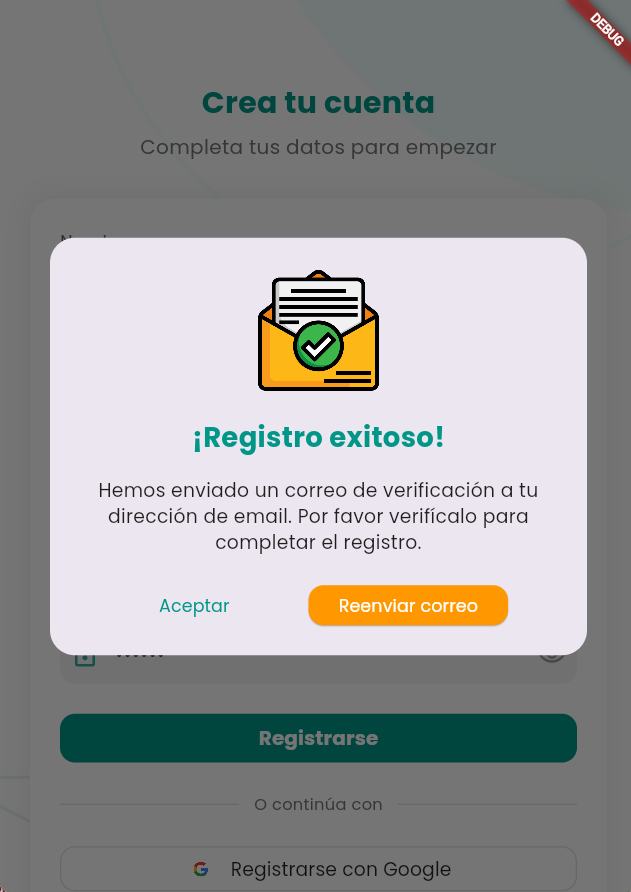
\includegraphics[width=0.55\textwidth]{../capitulos/img/manual3.png}
        \caption{Pantalla de verificación de correo electrónico}
\end{figure}

Antes de pulsar una de las opciones, debemos ir a nuestro correo electrónico y buscar el correo de verificación enviado por la aplicación.
En caso de que no lo recibamos, debemos revisar la carpeta de \textit{Spam} o \textit{Correo no deseado}.
Si no se recibe el correo, podemos pulsar el botón de \textit{Reenviar correo} para que se vuelva a enviar el correo de verificación.

Una vez recibido el correo, debemos pulsar el enlace de verificación que nos mostrará una pantalla de confirmación de que nuestra cuenta ha sido verificada correctamente.

Una vez realizada la verificación, podemos volver a la aplicación y pulsar el botón de \textit{Aceptar} para regresar a la pantalla de inicio de sesión.


Hay otra opción para registrarse, que es a través de una cuenta de Google. Para ello, debemos pulsar el botón de \textit{Registrarse con Google} que nos llevará a una pantalla de inicio de sesión de Google, donde debemos introducir nuestras credenciales de Google (correo electrónico y contraseña) para iniciar sesión.

Una vez iniciada la sesión, se nos pedirá que otorguemos permisos a la aplicación para acceder a nuestra cuenta de Google. Debemos aceptar los permisos para completar el registro.

\subsection*{Inicio de sesión}

A esta pantalla podemos acceder o bien desde la pantalla de bienvenida, o bien una vez registrados como se ha explicado anteriormente.
En ambos casos, el proceso es el mismo. Debemos introducir nuestro correo electrónico y contraseña en los campos correspondientes y pulsar el botón de \textit{Iniciar sesión}.

\begin{figure}[H]
    \centering
        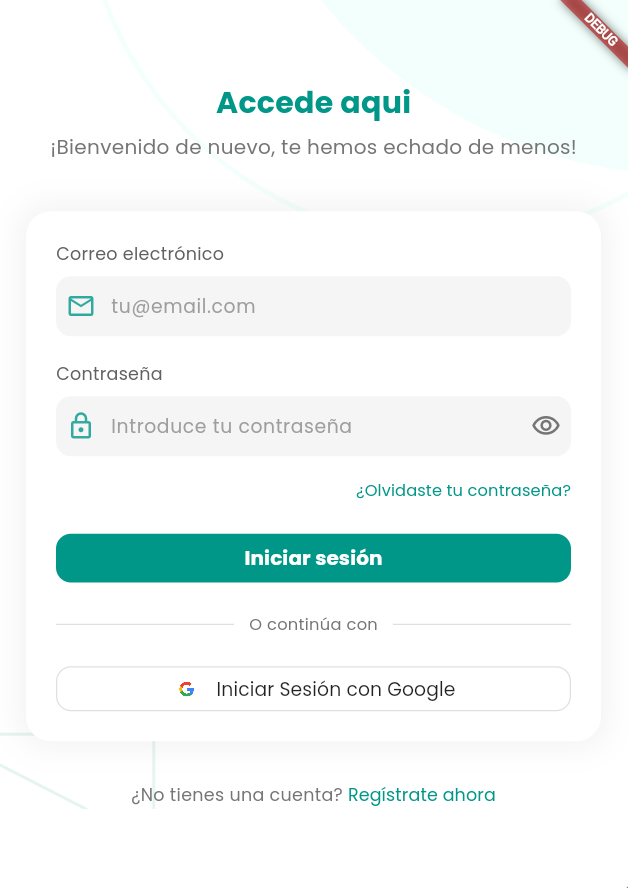
\includegraphics[width=0.55\textwidth]{../capitulos/img/inicio_sesion_implementado.png}
        \caption{Pantalla de inicio de sesión}
\end{figure}

En caso de que no hayamos verificado nuestra cuenta, se nos mostrará un mensaje de error indicando que debemos verificar nuestra cuenta antes de iniciar sesión. En este caso, debemos seguir el proceso de verificación descrito anteriormente.

\begin{figure}[H]
    \centering
        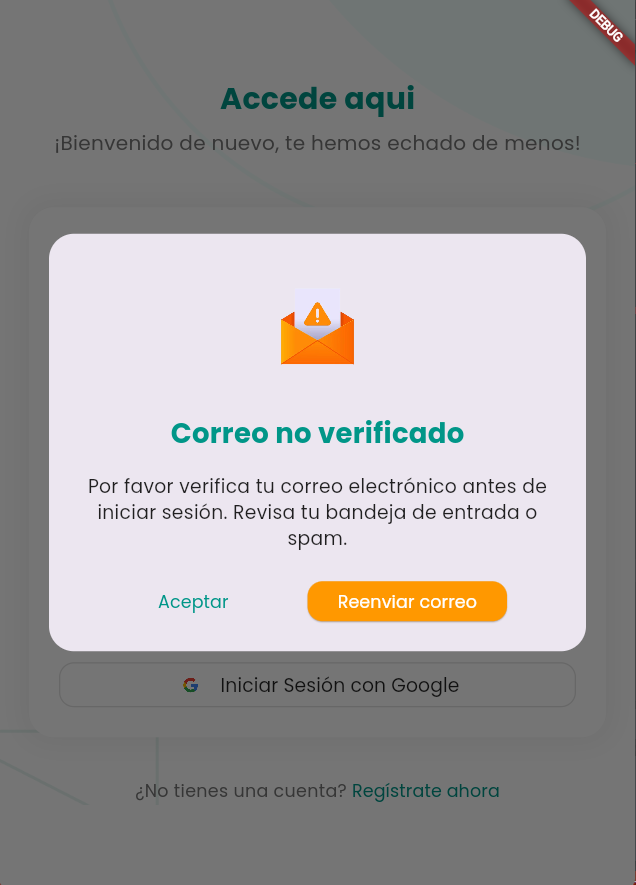
\includegraphics[width=0.55\textwidth]{../capitulos/img/manual4.png}
        \caption{Pantalla principal tras iniciar sesión sin verificar la cuenta}
\end{figure}

Tenemos la opción de iniciar sesión con una cuenta de Google, pulsando el botón de \textit{Iniciar sesión con Google}. Esto nos llevará a la pantalla de inicio de sesión de Google, donde debemos introducir nuestras credenciales de Google (correo electrónico y contraseña) para iniciar sesión.
En caso de ya nos hubiéramos registrado con una cuenta de Google, se iniciará sesión directamente, en caso contrario, se nos creará una cuenta nueva con los datos de nuestra cuenta de Google.

\begin{figure}[H]
    \centering
        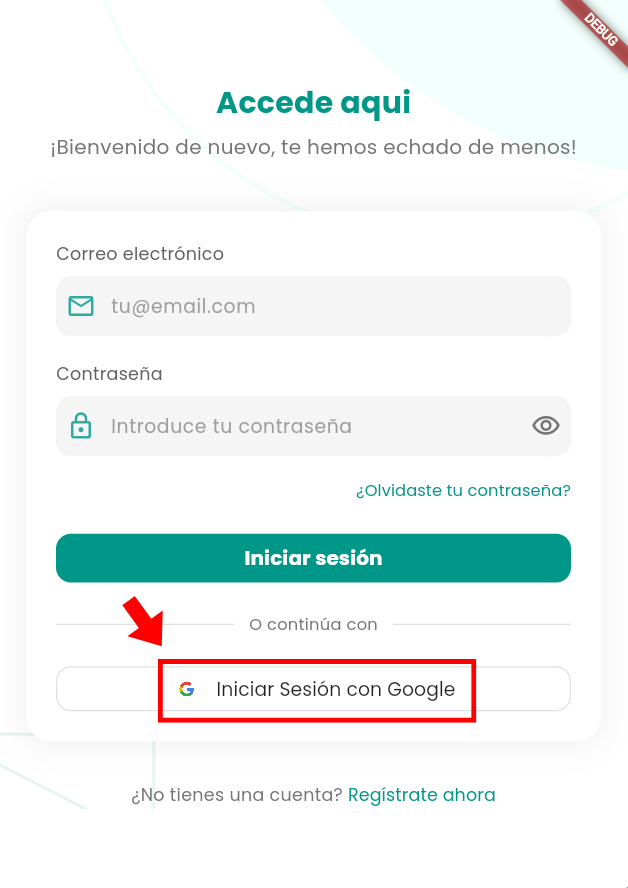
\includegraphics[width=0.55\textwidth]{../capitulos/img/manual5.png}
        \caption{Opción de iniciar sesión con Google}
\end{figure}

Una vez realizado estos pasos, habremos iniciado sesión correctamente.

\newpage


\section{Gestión del hogar}

Al iniciar sesión por primera vez o al abandonar un hogar, se nos mostrar la siguiente pantalla, donde se nos ofrecen dos opciones, crear un nuevo hogar o unirse a un hogar existente.
El hogar es el espacio compartido donde se gestionarán las tareas, gastos y listas de la compra. Cada hogar tiene un código único lo que permite 
que solo los miembros del hogar puedan acceder a la información y funcionalidades de dicho hogar.

\begin{figure}[H]
    \centering
        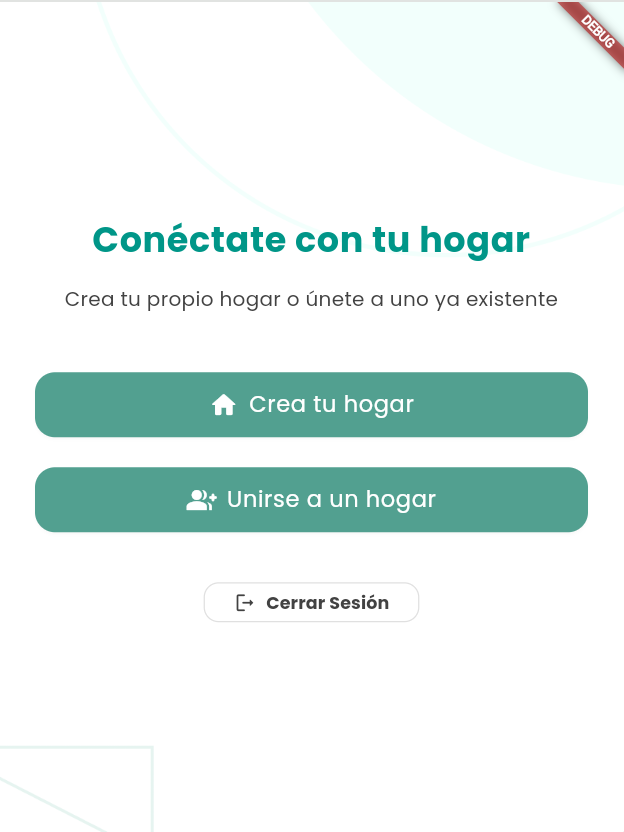
\includegraphics[width=0.55\textwidth]{../capitulos/img/opciones_impletementado.png}
        \caption{Pantalla de gestión del hogar} 
\end{figure}

Si alguien con el que compartes hogar ya ha creado un hogar, te proporcionará el código de dicho hogar para que puedas unirte a él. En ese caso 
selecciona la opción de \textit{Unirse a un hogar} y escribe el código de acceso que te ha proporcionado tu compañero de piso.

\begin{figure}[H]
    \centering
        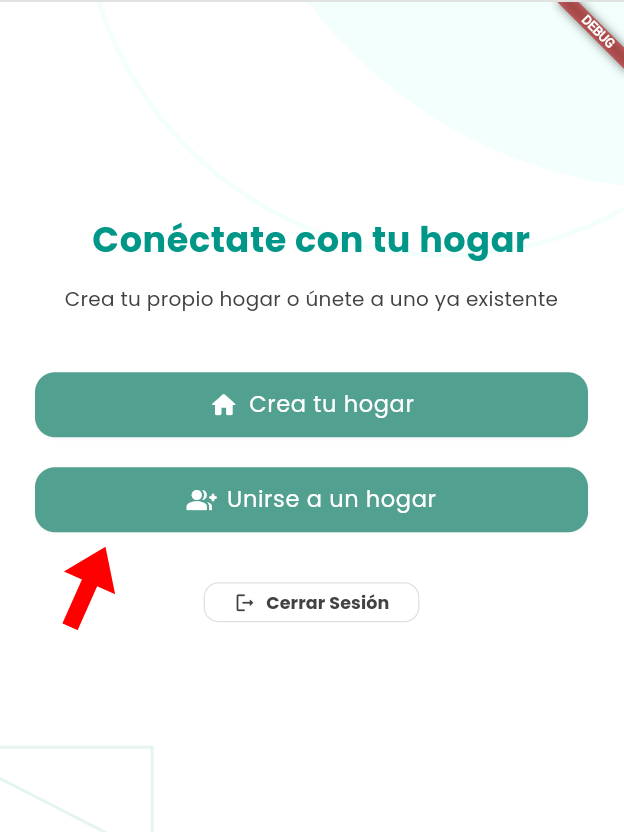
\includegraphics[width=0.55\textwidth]{../capitulos/img/manual6.png}
        \caption{Opción de unirse a un hogar}
\end{figure}

Una vez introducido el código de acceso, hay que pulsar el botón de \textit{Verificar código} para unirse al hogar. Si el código es correcto, se te añadirá al hogar y podrás acceder a todas las funcionalidades del mismo.
Si el código es incorrecto, se te mostrará un mensaje de error indicando que el código no es válido. En ese caso, debes asegurarte de que has introducido el código correctamente o pedir a tu compañero de piso que te proporcione el código correcto.

\begin{figure}[H]
    \centering
        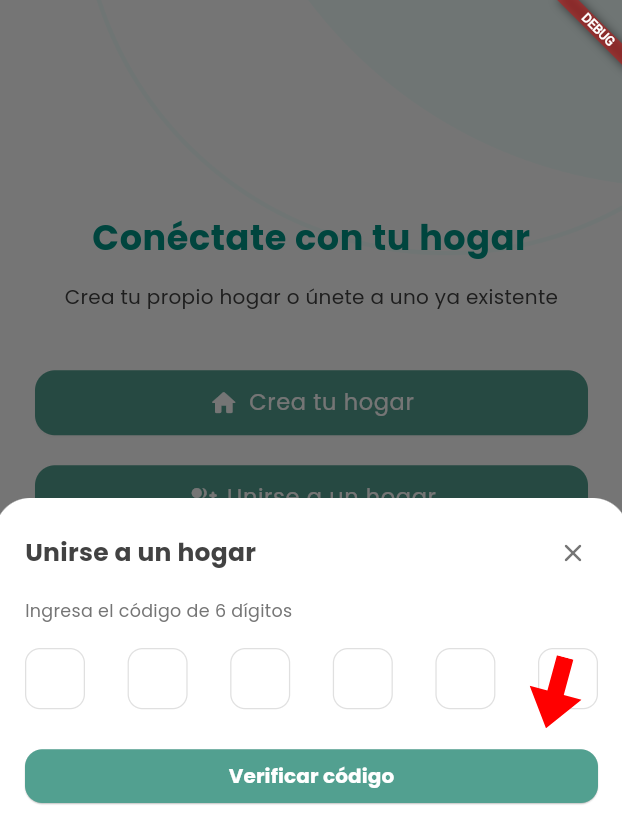
\includegraphics[width=0.55\textwidth]{../capitulos/img/manual7.png}
        \caption{Opción verificar código de acceso}
\end{figure}

Si eres el encargado de crear el hogar, debes pulsar el botón de \textit{Crea tu hogar} para crear un nuevo hogar. 

\begin{figure}[H]
    \centering
        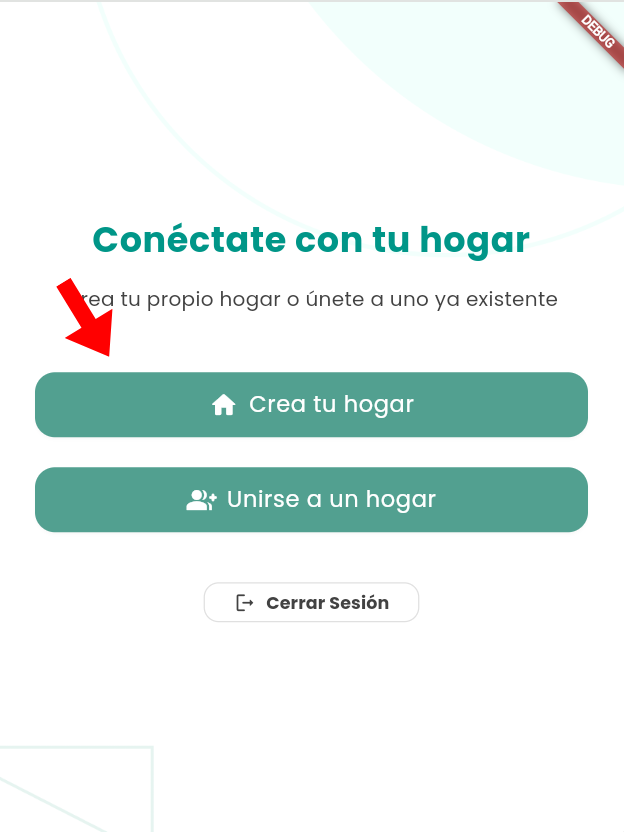
\includegraphics[width=0.55\textwidth]{../capitulos/img/manual8.png}
        \caption{Opción de crear de un nuevo hogar}
\end{figure}

Una vez elegida esta opción, se te pedirá que introduzcas un nombre para el hogar. Este nombre será visible para todos los miembros del hogar y se utilizará para identificar el hogar en la aplicación.
Es obligatorio introducir un nombre para el hogar y una vez introducido, debes pulsar el botón de \textit{Crear hogar} para crear el hogar.

\begin{figure}[H]
    \centering
        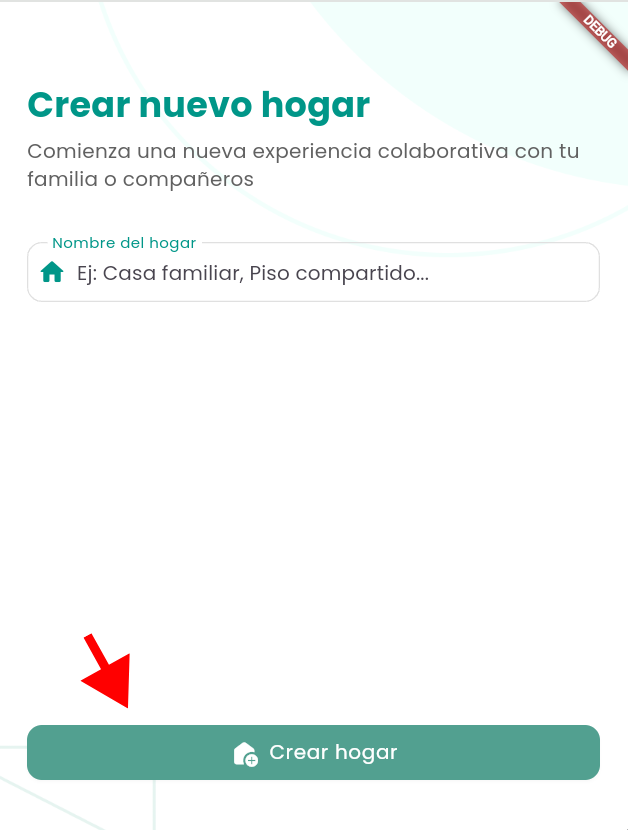
\includegraphics[width=0.55\textwidth]{../capitulos/img/manual9.png}
        \caption{Pantalla de creación de un nuevo hogar}
\end{figure}

Una vez realizado correctamente uno de los dos procesos anteriores, se te llevará a la pantalla principal de la aplicación.

\newpage

\section{Pantalla principal y navegación}



\section{Gestión de tareas}

\section{Gestión de gastos}

\section{Listas de la compra}

\section{Perfil de usuario y configuración}

